The first chapter introduces the context and the main concepts of a digital twin (DT), followed by describing the current challenges associated with integration and orchestration of models in a DT. This leads to the motivation for constructing a microbrewery case study in order to investigate frameworks for integration and orchestration.

The DT concept was first introduced by Grieves in 2002 \cite{Grieves2019}. He referred to it as a concept for Product Lifecycle Management (PLM). The concept asserts that systems are dual in nature, that is, a system has a physical side and a virtual side. The premise of the model is that the two sides are bound together via a bidirectional data link.

The association to PLM is that a DT is a dynamic system that adapts to specific stages in the product's lifecycle. The stage changes made in either space are promptly translated to the subsequent outcomes in the other space. For example, the physical product may deliver data about itself or the environment to the virtual space. On the other end, the developer could tune the design on the virtual side, resulting in calibration of the physical product. This bidirectional relationship in DTs makes a clear distinction from simulations, which are frequently confused with DTs. In short, we consider that DTs go a step further by using simulations and analyses to influence the outcomes in physical space.

After Grieves' proposal of using DTs for PLM, the early adopters were from the aerospace sectors such as NASA and US Air Force \cite{Grieves2019}. The lifecycle of an aircraft normally lasts several decades \cite{boeing}. Taking a single snapshot, an aircraft is a complex composition of multi-disciplinary outputs. For instance, the jet engine is a mechanical system; the fuel system is largely based on chemical reactions; and the communication equipment is the result of electrical and computer designs. The aerospace industry has shown the utility of DTs regarding products with a broad development scale. As time passed, many more industries quickly caught up with the trend of multi-disciplinary and long-term product lifecycle. Production factories these days use dedicated software to analyze the efficiency of operations and optimize them on-the-go \cite{Zheng2018}. Hospitals also use digital assets to aid experiments on drugs and patients \cite{Kwon2022}. As a result, the study of DT development becomes more and more important.

The number and variety of DTs continue to expand these days. In the physical space, this is attributed to advancements---alongside reduction of costs---in wireless sensor networks. In the virtual space, more sophisticated modeling methods are appearing; especially, there has been a rapid progress in big-data models and artificial intelligence models \cite{Duan2019}. Under this premise we notice a problem of how to manage all the available components together in a DT in order to support the product lifecycle. To have heterogeneous tools cooperating we need integration and orchestration. These two notions include aspects as focused as data format conversion, as well as bigger considerations like inter-model scheduling. We want to investigate what are the key characteristics for integration and orchestration. 

Identifying the integration and orchestration techniques is merely the first step to improve a DT development process. Applied separately, individual techniques can hardly reduce the complexity of the process on their own. They need to be arranged in a coherent order and be governed together by operating principles. This is why we need to experiment with different frameworks for integration and orchestration in this project. A framework, simply speaking, embodies these techniques and consolidates them into a certain workflow pattern, laying out a guideline for a developer to follow. Adopting a framework when constructing DTs also ensures good practices could be reproduced consistently, as it encourages common resource utilization, for instance, through templates or libraries. Alternatively, workflow stages could also be established in the framework as discussed in the later chapters. 

An end goal of a DT is to support services in a product lifecycle. In this project we want to search for what approaches, offered by the frameworks, have the potential to enable accomplishing this goal. We choose a microbrewery as the case study, the core services we will focus on are related to the production yield aspect of the beer. A key process of a brewery is fermentation, which typically spans two weeks. The process has various variables that could be monitored by sensors, such as the alcoholic content and the temperature. Moreover, the conditions of the process are relatively mild, i.e., low temperature, medium high pressure, which allows easy observations. The fermentation process is a well studied phenomenon, making it straightforward to construct and evaluate. Taken together, these conditions within the case study give us great flexibility to test the different frameworks. 

\section{Context}\label{sec:context}
As claimed by market analysts \cite{pwc2014, ibm}, the emerging trend of Industry 4.0 is characterized by widespread digitalization. Hence DTs are becoming more widely adopted as industry moves toward a digital transformation which sets out to improve the transfer of information across the value chain. This will allow stakeholders to share knowledge about the designs, conditions, and logistics of their products and operations through digital artifacts. By facilitating the virtual mock-up of the real product, one can overcome the temporal and spatial limitations of experimenting in the physical world, thus greatly reducing the overall cost.

The concept of DT is often discussed together with the model-driven system engineering (MDSE) paradigm \cite{Bordeleau2020}. In MDSE, a complex system is treated holistically. It is described in terms of the interaction between systems, or better known as ``system of systems" \cite{Kossiakoff2011}. The system architecture is represented as models in order to support requirements, design, analysis and verification activities throughout the lifecycle. The use of modelling exploits recurring design patterns, hence helping to drive a consistent specification without significantly increasing costs as the system depth---the total number of abstraction layers---extends. It is found in many studies that DTs which follow MDSE have the potential to bring the following benefits \cite{Boschert2016, Macchi2018, Lim2019, Ansari2020, Cai2021, Gurdur2022}:
\begin{itemize}
  \item Reduced maintenance costs during a system's lifecycle.
  \item Reduced errors and inconsistencies across multiple iterations. 
  \item Improved multi-disciplinary collaboration, i.e., engineers from different job functions are able to quickly grasp the high-level overview of the design.
\end{itemize}

\section{Domain overview}\label{sec:overview}
In this section we first discuss the DT classification. After that, we provide an overview a five-dimensional view of DT which helps us to assess the individual components and their interactions.
\subsubsection{Classification}
Although the term ``digital twin" has been mentioned in much literature, such studies seldomly share the same definition \cite{Liu2021}. In some studies the definition centers on to multi-scale simulations working together \cite{Shafto2012}. In other studies it is defined as a high fidelity digital replica of the physical asset \cite{Schluse2018}. In order to find a definition that fits our case study, and to keep the later discussions consistent, we will adopt the classification proposed by Kritzinger et al. \cite{Kritzinger2018}. According to the classification, `digital twin' can be roughly divided in three categories based on the level of data integration between the physical assets and their virtual counterpart (illustrated in Figure \ref{fig:dt}):

\begin{figure}[hbt!]
  \centering
  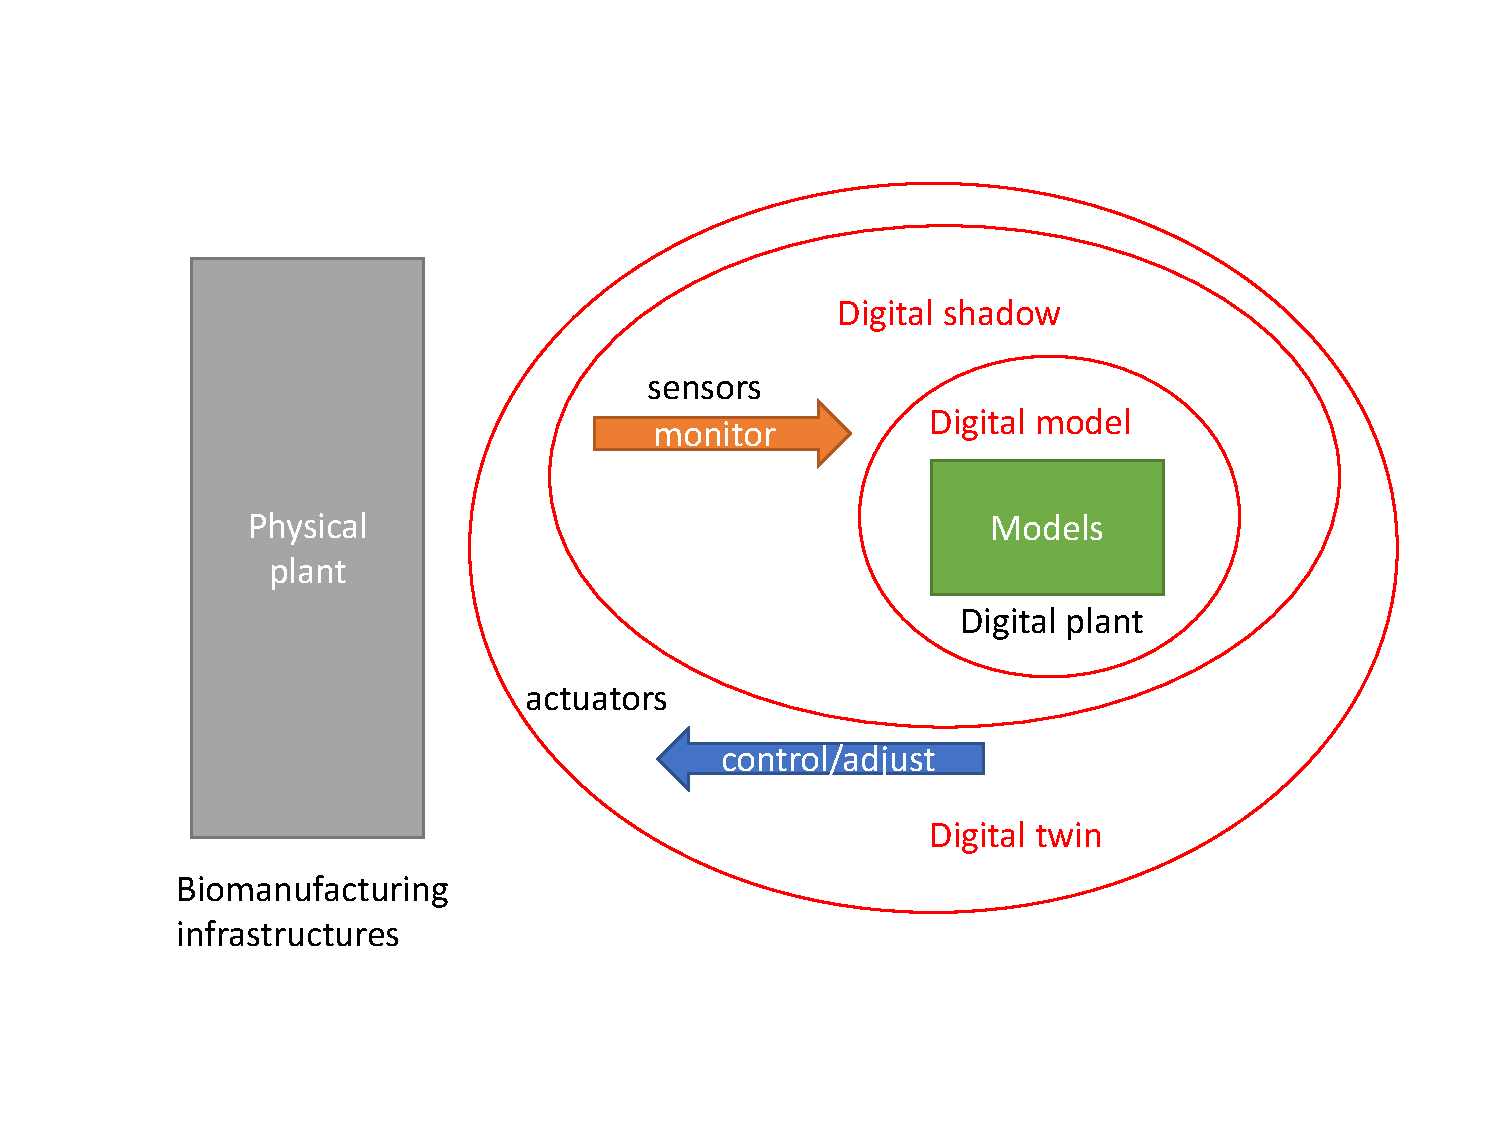
\includegraphics[scale=0.5]{figures/dt.pdf}
  \caption{Classification of digital twin}
  \label{fig:dt}
\end{figure}

\begin{itemize}

  \item \textbf{Digital model}: The virtual space does not involve data exchange with the physical space in an automated fashion. Hence the changes in one part have no direct effect on the other unless updates are performed manually.

  \item \textbf{Digital shadow}: There exists an automated one-way data communication from the physical object to the virtual one.
  
  \item \textbf{Digital twin}: Bi-directional data exchange between the physical space and the virtual space is automated. Changes made in the physical space will be reflected in the virtual space and vice versa. 

\end{itemize}

In a manufacturing plant setting, data delivered from the physical world to the virtual world is used for monitoring. The reverse direction amounts to the adjustments of actuators. It is important to note that adjusting an actuator in a DT often has a different connotation with the traditional control scheme. In an old-fashioned control style, the computed value is sent to the actuator as a direct activation of certain operations; whereas in a DT, the computed values more likely belong to the parameter set of a complex controlling model that influence the actuators in more nuances, such as adjusting the weighting factors.

A fully automated DT might be unfeasible in certain domains. In particular, for the bio-chemical domain, Udugama et al. \cite{Udugama2020, Udugama2021} recognize that human interventions are still necessary in many scenarios. In practice, it is often the case that DTs deliver the suggestions to the operator through a human machine interface (HMI) first; and the operator can act on the available data. This concept is called human-in-the-loop, and is demonstrated in \cite{Barricelli2020} for an athlete DT, where the coach manages the fitness plan for the athlete based on the reports given by the DT. Since this project concerns a microbrewery which also lies in the bio-chemical domain, the relaxed definition of DT is considered relevant.    

Another variant of DT workflow which specifically targets the bioprocessing theme is introduced in \cite{Udugama2021}. One might find the alternative relevant if the DT includes a multitude of static and dynamic chemical processes. More details can be found in Appendix \ref{apd:workflow}.

\subsubsection{Dimension}
This section introduces a DT model by Tao et al. \cite{Tao2017}, focusing on the interconnections between different parts. They propose a five-dimensional view of DT model shown in Figure \ref{fig:tao5d}. Each dimension is described as follows:

\begin{figure}[hbt!]
  \centering
  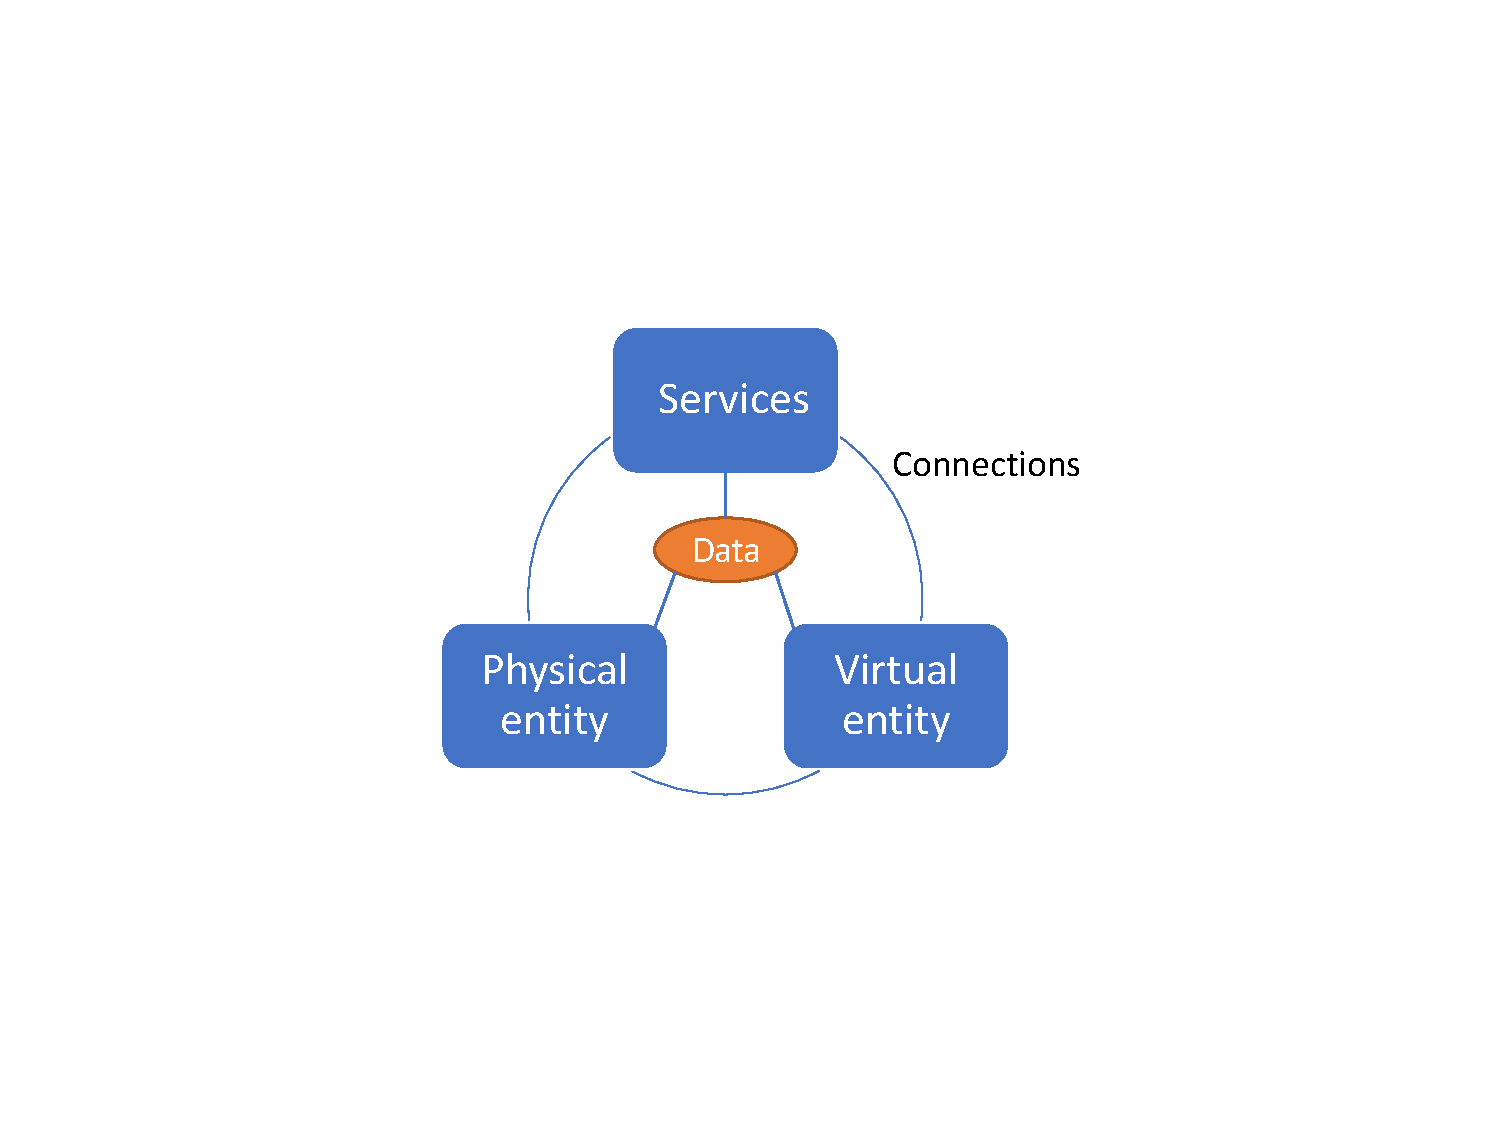
\includegraphics[scale=0.5]{figures/tao5d.pdf}
  \caption{5D view of DT model}
  \label{fig:tao5d}
\end{figure}

\begin{itemize}

  \item \textbf{Physical entity} (PE): A collection of sensors and equipment working collaboratively to collect real-time data for the intended services, meanwhile receiving control orders from the virtual world.    

  \item \textbf{Virtual entity} (VE): A digital mirror, which contains models simulating the physical counterpart with high fidelity. Calibration strategies are generated through comparing the models with entities to support models' evolution.
  
  \item \textbf{Services}: Provides various services to support the management and control of PEs as well as the operation and evolution of VEs. Services are usually requested by the users to fulfill certain functionalities.
       
  \item \textbf{Data}: A shared storage consisting of the raw data from PEs, VEs, and services. It may also be responsible for merging data from various sources to a fused format. 
   
  \item \textbf{Connections}: The connections for all four of the above-mentioned dimensions. Relevant concepts include communication protocols, access ports, etc.
  
\end{itemize}

As we can see the five elements form separate dimensions, yet it has to be ensured that they can inter-operate correctly and effectively. A main goal of integration and orchestration is to address this issue. In particular, the interoperability among VEs is what we will concentrate most on in this project, for the reason explained in the following section. 


\section{Challenges}\label{sec:challenges}
This section describes the difficulty of managing multiple models in a DT. We give explanations of why the solutions available in commercial platforms are insufficient. Hence it motivates us to look for frameworks that address the challenges. We also acknowledge that generalizing the approaches is equally important as solving for the specific microbrewery case study.

As DTs become increasingly powerful and used for complex systems, diverse tools and heterogeneous models inevitably must be used to cover all aspects for DT constructions. In this step, the challenges in integration and orchestration arise. The terms integration and orchestration can be understood as:

\begin{itemize}

  \item \textbf{Integration} couples different models by \underline{encapsulating} their properties and operations, followed by \underline{interfacing} the abstract representations with a proper communication method.

  \item \textbf{Orchestration} dictates models' \underline{execution schedule} and arranges the \underline{event queue} for the events of a particular execution.

\end{itemize}

Commercial platforms like Simulink \cite{Simulink} or CATIA \cite{CATIA} tackle the issue by expanding their ecosystem with proprietary plugins and extensions so the users can rely less on external implementations. Although these platforms still have some third-party tool support---often by means of imports---they are not promoted as common practice, and the users are more likely encouraged to use the built-in toolbox for better reliability. In the work of van den Brand et al. \cite{brand2021}, a similar observation is mentioned, stating that many commercial frameworks support integration and orchestration only to a selective modeling toolset. Therefore, we need to find a framework that extends the support to more models.

The research on an open framework that incorporates integration and orchestration as fixtures in the design workflow remains scarce. As the number of models and their interactions increases, the complexity of control and data flows will grow significantly. Adopting a framework allows the integration and orchestration to scale proportionally, and be replicated consistently. This ultimately contributes to streamlining of DT developments.

Another study produced by Negrin et al. \cite{Negrin2021} investigated the integration and orchestration concerning an autonomous truck at a distribution center. This study signifies the importance of considering the specific DT's purpose and use case context, while extracting the universal properties of integration and orchestration which can be applied in other domains.

\section{Problem definition}\label{sec:prodef}
Figure \ref{fig:intorc} illustrates the main ideas which are covered by integration and orchestration respectively. On the right side, it shows that integration comprises two aspects, namely encapsulation and interface. Encapsulation refers to the abstraction of a model, as well as discerning the relevant inputs and outputs from the rest of internal operations of the model. The common notion of a ``black box" system is a form of encapsulation. This allows the interaction with other models to take place without redundancy while still retaining all necessary information. The interface, on the other hand, is responsible for building a bridge of communication agreed by the involving models, such that the correctness---both numerical and semantic---of data can be reliably maintained. A common way of interfacing is by using an established protocol, so all data transmissions will adhere to a fixed set of rules. 

\begin{figure}[hbt!]
  \centering
  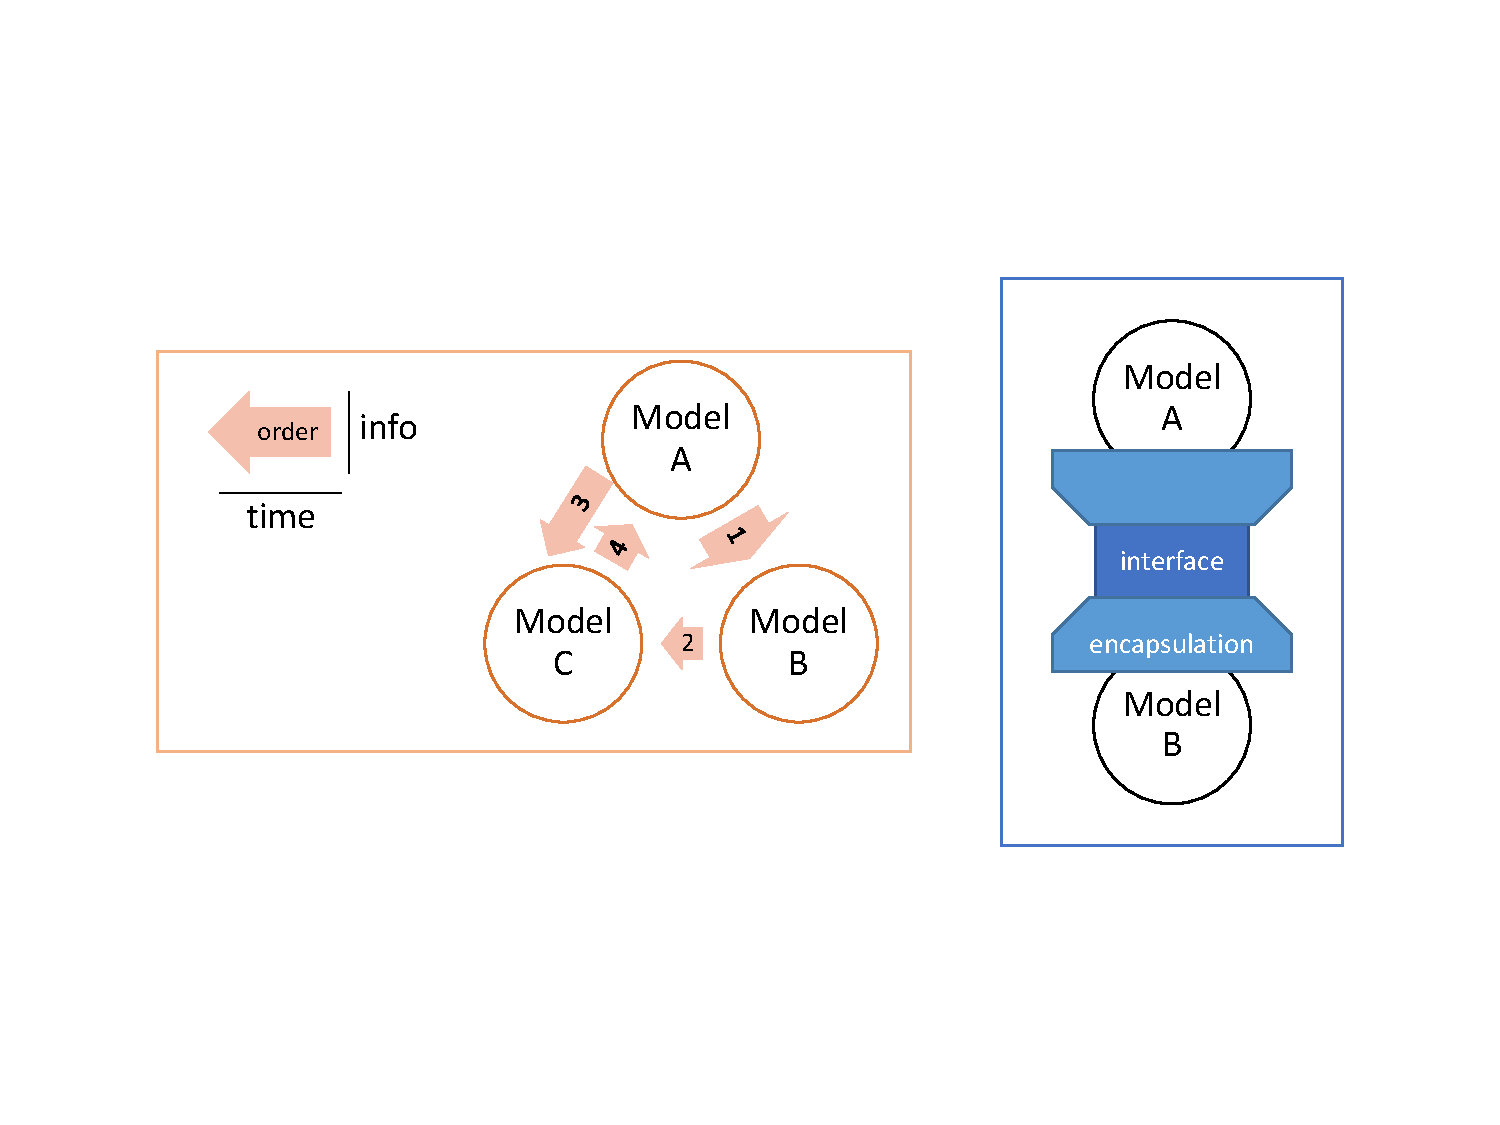
\includegraphics[scale=0.5]{figures/intorc.pdf}
  \caption{Integration (right) and orchestration (left)}
  \label{fig:intorc}
\end{figure}

On the left side, the concept of orchestration is shown. It encompasses two parts: (1) The scheduling relation between different models; in the figure it is represented by arrow shapes. The numbering in the arrows indicates the execution order. The difference in execution time incurred is represented by length variety of the arrow shapes. Furthermore, different information types may also be transferred from one model to another, whether it is a single trigger, or a stream of data, etc. The widths of the arrow shapes are used to highlight such discrepancy. (2) The handling of events, that is, the policy to control how event instances are accessed in the event queue \cite{Ptolemaeus2014}. In here the events refers to internal events of a particular execution. 

While (1) looks at individual model as an abstraction, (2) focuses on the task sequence within the model in order to ensure a deterministic outcome. A situation that might require event handling, is when several models are scheduled to execute concurrently, their respective events might arrive and leave in different order.

\section{Project Scope}\label{sec:scope}
This is an exploratory project of the possible frameworks for integration and orchestration techniques, supported by the implementation of the microbrewery DT as case study. 

The fermentation process models in the DT are given, they are developed by tutor Manrique Negrin, a hobby brewer and a chemist by training. Hence the details of these models or simulation algorithms are not within the scope. A comparative study of the three selected frameworks---detailed in Chapter \ref{ch:methodology}---will be conducted in parallel to the DT services development. Despite the considered use case being influenced by a bio-chemical theme, we strive to maintain universality in the analysis, such that the findings can be applied in other domains as well.

Functional and system level testing of the DT are also part of the implementation scope in order to evaluate the performance outcomes.

\section{Research questions}\label{sec:rqs}
Given the premises, in this study an attempt is made to answer the following research questions: 

\begin{itemize}

  \item \textbf{RQ1}: What are the key ingredients for integration and orchestration of models in different services for a microbrewery DT?
  \item \textbf{RQ2}: How can these ingredients be generalized to benefit other application domains? 
  \item \textbf{RQ3}: In what circumstances do the selected frameworks best fit these ingredients?  
  
\end{itemize}

Collectively, the answers to these research questions will lead to expanding our knowledge of: \textit{What are considered good practices for the integration and orchestration of DT models?}

\section{Report structure}
The rest of this report is structured as follows: 

\begin{itemize}

\item Chapter \ref{ch:background} presents the state of the art regarding the technologies that constitute a DT. We will also examine a number of related works which address the topic of integration and orchestration.

\item Chapter \ref{ch:methodology} describes the high-level architecture of the design process. The proposed services as well as their requirements and KPIs will be elicited. We will discuss the selected frameworks for integration and orchestration.

\item Chapter \ref{ch:implementation} describes the workflow of individual frameworks, from initial setup to resultant implementation.

\item Chapter \ref{ch:discussion} explains and compares the results between the frameworks, then summarizes the findings.

\item Chapter \ref{ch:conclusion} uses the findings to answers the research questions, and discusses future work.

\end{itemize}

